\documentclass[aspectratio=169,10pt,t]{beamer}
% 决赛展示 PPT 公共样式（Beamer，16:9，XeLaTeX）——商业路演稿标准
% 用法：
%   \documentclass[aspectratio=169,10pt,t]{beamer}   % t：内容顶端对齐，结论条压到页底
%   % 决赛展示 PPT 公共样式（Beamer，16:9，XeLaTeX）——商业路演稿标准
% 用法：
%   \documentclass[aspectratio=169,10pt,t]{beamer}   % t：内容顶端对齐，结论条压到页底
%   % 决赛展示 PPT 公共样式（Beamer，16:9，XeLaTeX）——商业路演稿标准
% 用法：
%   \documentclass[aspectratio=169,10pt,t]{beamer}   % t：内容顶端对齐，结论条压到页底
%   \input{../_style/slides_preamble.tex}
%   \title{…} \subtitle{…} \author{fx战队} \date{2026 年 11 月}
%   \TrackName{因子赛道}
%
% 页面结构：结论标题（浅显） + 主体（图 / 示意图 / 表 / 要点块） + 底部结论条 \takeaway{…}
% 组件：\ChapterFrame、\keynum、\point、panel 环境、\takeaway、\hl

\usepackage[fontset=none,scheme=plain]{ctex}
% 字体：微软雅黑（取自本机 Office 安装包，不复制进仓库），大号数字用 DIN
\def\yhpath{/Applications/Microsoft PowerPoint.app/Contents/Resources/DFonts/}
\setCJKmainfont{msyh.ttc}[Path=\yhpath,BoldFont=msyhbd.ttc]
\setCJKsansfont{msyh.ttc}[Path=\yhpath,BoldFont=msyhbd.ttc]
\setCJKmonofont{msyh.ttc}[Path=\yhpath]
\newCJKfontfamily\titlecjk{msyhbd.ttc}[Path=\yhpath]
\setsansfont{msyh.ttc}[Path=\yhpath,BoldFont=msyhbd.ttc]
\setmainfont{msyh.ttc}[Path=\yhpath,BoldFont=msyhbd.ttc]
\newfontfamily\titlelatin{msyhbd.ttc}[Path=\yhpath]
\newfontfamily\numfont{DIN Alternate}
\usefonttheme{professionalfonts}

\usepackage{newunicodechar}
\newunicodechar{→}{\ensuremath{\rightarrow}}
\newunicodechar{↑}{\ensuremath{\uparrow}}
\newunicodechar{↓}{\ensuremath{\downarrow}}
\newunicodechar{≈}{\ensuremath{\approx}}
\newunicodechar{≤}{\ensuremath{\leq}}
\newunicodechar{≥}{\ensuremath{\geq}}
\newunicodechar{−}{\ensuremath{-}}
\newunicodechar{×}{\ensuremath{\times}}
\newunicodechar{÷}{\ensuremath{\div}}
\newunicodechar{±}{\ensuremath{\pm}}
\newunicodechar{β}{\ensuremath{\beta}}
\newunicodechar{λ}{\ensuremath{\lambda}}

% 配色：深蓝主色、橙色强调、浅蓝底色
\definecolor{snavy}{HTML}{0F2E5A}
\definecolor{sblue}{HTML}{2F6DB5}
\definecolor{stint}{HTML}{E8EFF8}
\definecolor{sorange}{HTML}{E8772E}
\definecolor{sgrey}{HTML}{5E6672}
\definecolor{sline}{HTML}{C9D3E0}
\definecolor{sink}{HTML}{1E2329}

\setbeamercolor{normal text}{fg=sink,bg=white}
\setbeamercolor{structure}{fg=snavy}
\setbeamercolor{frametitle}{fg=snavy}
\setbeamercolor{alerted text}{fg=sorange}
\setbeamertemplate{navigation symbols}{}
\setbeamertemplate{itemize items}{\textcolor{sblue}{\rule[0.25ex]{0.42em}{0.42em}}}
\setlength{\leftmargini}{1.1em}
\linespread{1.18}
\setbeamersize{text margin left=1.0cm, text margin right=1.0cm}
% 内容顶端对齐，结论条用 \vfill 压到页底
\makeatletter\beamer@centeredfalse\makeatother

\providecommand{\trackname}{}
\gdef\chaplabel{}
\newcommand{\TrackName}[1]{\renewcommand{\trackname}{#1}}

\usepackage{tikz}
\usetikzlibrary{arrows.meta,positioning,calc,fit,decorations.pathreplacing,shapes.geometric}

% 顶部深蓝细带 + 标题左侧橙色色块 + 右上章节标签
\setbeamertemplate{frametitle}{%
  \begin{tikzpicture}[remember picture,overlay]
    \fill[snavy] (current page.north west) rectangle ([yshift=-0.12cm]current page.north east);
  \end{tikzpicture}%
  \vspace*{0.36cm}%
  \begin{minipage}[c]{0.80\textwidth}%
    {\color{sorange}\rule[-0.05cm]{0.13cm}{0.52cm}}\hspace{0.22cm}%
    {\titlelatin\titlecjk\color{snavy}\fontsize{16pt}{20pt}\selectfont\insertframetitle}%
  \end{minipage}\hfill
  \ifx\chaplabel\empty\else
  \begin{tikzpicture}[baseline=-0.6ex]
    \node[fill=snavy,text=white,rounded corners=1.5pt,inner xsep=6pt,inner ysep=3pt,font=\footnotesize]{\chaplabel};
  \end{tikzpicture}\fi\par
  \vspace{0.25cm}}

% 页脚：只有页码
\setbeamertemplate{footline}{\hfill{\numfont\color{sgrey}\small\insertframenumber}\hspace*{0.6cm}\vspace*{0.3cm}}

\usepackage{appendixnumberbeamer}

% ---------- 组件 ----------
\newcommand{\hl}[1]{\textcolor{sorange}{\bfseries #1}}
% 大号关键数字：\keynum{0.290}{换手率（原 0.518）}
\newcommand{\keynum}[2]{%
  \begin{minipage}[t]{\linewidth}\raggedright
    {\numfont\color{sorange}\fontsize{26pt}{28pt}\selectfont #1}\par\vspace{0.06cm}
    {\color{sink}\small #2}\par
  \end{minipage}}
% 编号要点：\point{1}{加粗短句}{一两句解释}
\newcommand{\point}[3]{%
  \begin{tikzpicture}[baseline=(n.base)]
    \node[circle,fill=snavy,text=white,inner sep=1.6pt,minimum size=0.48cm,font=\numfont\small](n){#1};
  \end{tikzpicture}\hspace{0.18cm}%
  \begin{minipage}[t]{\dimexpr\linewidth-0.75cm\relax}
    {\bfseries\color{snavy}#2}\par\vspace{0.03cm}{\small\color{sink}#3}
  \end{minipage}\par\vspace{0.16cm}}
% 浅蓝底面板：\begin{panel}{标题} … \end{panel}
\newenvironment{panel}[1]{%
  \par\noindent\begin{tikzpicture}\node[fill=stint,rounded corners=2pt,inner sep=8pt,text width=\dimexpr\linewidth-16pt\relax,align=flush left]\bgroup
  {\bfseries\color{snavy}#1}\par\vspace{0.12cm}\small}
  {\egroup;\end{tikzpicture}\par}
% 底部结论条：一句话说明这一页证明了什么（固定在页底，正文不要压到这一区域）
\newcommand{\takeaway}[1]{%
  \begin{tikzpicture}[remember picture,overlay]
    \node[fill=snavy,text=white,inner xsep=10pt,inner ysep=6pt,anchor=south,
          text width=\dimexpr\paperwidth-2cm-20pt\relax,align=flush left,font=\small]
      at ([yshift=0.75cm]current page.south) {#1};
  \end{tikzpicture}}

% 表格
\usepackage{booktabs,tabularx,array,colortbl}
\renewcommand{\arraystretch}{1.32}
\newcolumntype{L}{>{\raggedright\arraybackslash}X}
\newcolumntype{C}{>{\centering\arraybackslash}X}
\newcommand{\headrow}{\rowcolor{snavy}}
\newcommand{\thc}[1]{\textcolor{white}{\bfseries #1}}
\newcommand{\ourrow}{\rowcolor{stint}}

% 图形
\usepackage{graphicx}
\usepackage{pgfplots}
\pgfplotsset{compat=1.18,tick label style={font=\numfont\small},label style={font=\small},/pgf/number format/assume math mode=true}
\tikzset{
  node/.style  = {draw=snavy, line width=0.8pt, fill=white, rounded corners=2pt, align=flush center,
                  inner xsep=7pt, inner ysep=5pt, font=\small},
  fillnode/.style = {fill=snavy, text=white, rounded corners=2pt, align=flush center,
                  inner xsep=7pt, inner ysep=5pt, font=\small\bfseries},
  tintnode/.style = {fill=stint, draw=none, rounded corners=2pt, align=flush center,
                  inner xsep=7pt, inner ysep=5pt, font=\small},
  key/.style   = {node, draw=sorange, line width=1.1pt},
  flow/.style  = {-{Stealth[length=2.6mm]}, line width=0.9pt, draw=snavy},
  note/.style  = {font=\small, text=sgrey, align=flush center},
}

% 封面：深蓝满版
\setbeamertemplate{title page}{%
  \begin{tikzpicture}[remember picture,overlay]
    \fill[snavy] (current page.south west) rectangle (current page.north east);
    \fill[sorange] ([xshift=1.2cm,yshift=-2.3cm]current page.north west) rectangle ++(1.6cm,0.12cm);
    \node[anchor=north west,text=white,text width=0.78\paperwidth,align=flush left]
      at ([xshift=1.2cm,yshift=-2.7cm]current page.north west)
      {{\titlecjk\fontsize{25pt}{33pt}\selectfont\inserttitle}\par\vspace{0.45cm}
       {\large\color{white!80!snavy}\insertsubtitle}};
    \node[anchor=south west,text=white,text width=0.6\paperwidth,align=flush left]
      at ([xshift=1.2cm,yshift=1.1cm]current page.south west)
      {{\large\bfseries\insertauthor}\par\vspace{0.12cm}{\small\color{white!75!snavy}\trackname\quad\insertdate}};
  \end{tikzpicture}}

% 章节页：深蓝满版，左侧大号编号与本章要回答的问题，右侧故事进度
\providecommand{\ChapterList}[1]{}
\newcommand{\ChapterFrame}[4]{%
  \section[#1\enspace #2]{#3}\gdef\chaplabel{#1\enspace #2}
  {\setbeamertemplate{footline}{}
  \begin{frame}[plain,noframenumbering]
    \begin{tikzpicture}[remember picture,overlay]
      \fill[snavy] (current page.south west) rectangle (current page.north east);
      \node[anchor=north west,text=white,text width=0.46\paperwidth,align=flush left]
        at ([xshift=1.2cm,yshift=-2.0cm]current page.north west)
        {{\numfont\color{sorange}\fontsize{48pt}{50pt}\selectfont #1}\par\vspace{0.35cm}
         {\titlecjk\fontsize{20pt}{26pt}\selectfont #3}\par\vspace{0.4cm}
         {\normalsize\color{white!85!snavy}#4}};
      \node[anchor=north west,text=white,text width=0.36\paperwidth,align=flush left]
        at ([xshift=0.58\paperwidth,yshift=-2.1cm]current page.north west)
        {\ChapterList{#1}};
    \end{tikzpicture}
  \end{frame}}}
\newcommand{\chapitem}[3]{\ifnum#1=#2{\color{white}\bfseries #2\enspace #3}\else{\color{white!55!snavy}#2\enspace #3}\fi\par\vspace{0.3cm}}

\hypersetup{colorlinks=true, linkcolor=snavy, urlcolor=snavy}

%   \title{…} \subtitle{…} \author{fx战队} \date{2026 年 11 月}
%   \TrackName{因子赛道}
%
% 页面结构：结论标题（浅显） + 主体（图 / 示意图 / 表 / 要点块） + 底部结论条 \takeaway{…}
% 组件：\ChapterFrame、\keynum、\point、panel 环境、\takeaway、\hl

\usepackage[fontset=none,scheme=plain]{ctex}
% 字体：微软雅黑（取自本机 Office 安装包，不复制进仓库），大号数字用 DIN
\def\yhpath{/Applications/Microsoft PowerPoint.app/Contents/Resources/DFonts/}
\setCJKmainfont{msyh.ttc}[Path=\yhpath,BoldFont=msyhbd.ttc]
\setCJKsansfont{msyh.ttc}[Path=\yhpath,BoldFont=msyhbd.ttc]
\setCJKmonofont{msyh.ttc}[Path=\yhpath]
\newCJKfontfamily\titlecjk{msyhbd.ttc}[Path=\yhpath]
\setsansfont{msyh.ttc}[Path=\yhpath,BoldFont=msyhbd.ttc]
\setmainfont{msyh.ttc}[Path=\yhpath,BoldFont=msyhbd.ttc]
\newfontfamily\titlelatin{msyhbd.ttc}[Path=\yhpath]
\newfontfamily\numfont{DIN Alternate}
\usefonttheme{professionalfonts}

\usepackage{newunicodechar}
\newunicodechar{→}{\ensuremath{\rightarrow}}
\newunicodechar{↑}{\ensuremath{\uparrow}}
\newunicodechar{↓}{\ensuremath{\downarrow}}
\newunicodechar{≈}{\ensuremath{\approx}}
\newunicodechar{≤}{\ensuremath{\leq}}
\newunicodechar{≥}{\ensuremath{\geq}}
\newunicodechar{−}{\ensuremath{-}}
\newunicodechar{×}{\ensuremath{\times}}
\newunicodechar{÷}{\ensuremath{\div}}
\newunicodechar{±}{\ensuremath{\pm}}
\newunicodechar{β}{\ensuremath{\beta}}
\newunicodechar{λ}{\ensuremath{\lambda}}

% 配色：深蓝主色、橙色强调、浅蓝底色
\definecolor{snavy}{HTML}{0F2E5A}
\definecolor{sblue}{HTML}{2F6DB5}
\definecolor{stint}{HTML}{E8EFF8}
\definecolor{sorange}{HTML}{E8772E}
\definecolor{sgrey}{HTML}{5E6672}
\definecolor{sline}{HTML}{C9D3E0}
\definecolor{sink}{HTML}{1E2329}

\setbeamercolor{normal text}{fg=sink,bg=white}
\setbeamercolor{structure}{fg=snavy}
\setbeamercolor{frametitle}{fg=snavy}
\setbeamercolor{alerted text}{fg=sorange}
\setbeamertemplate{navigation symbols}{}
\setbeamertemplate{itemize items}{\textcolor{sblue}{\rule[0.25ex]{0.42em}{0.42em}}}
\setlength{\leftmargini}{1.1em}
\linespread{1.18}
\setbeamersize{text margin left=1.0cm, text margin right=1.0cm}
% 内容顶端对齐，结论条用 \vfill 压到页底
\makeatletter\beamer@centeredfalse\makeatother

\providecommand{\trackname}{}
\gdef\chaplabel{}
\newcommand{\TrackName}[1]{\renewcommand{\trackname}{#1}}

\usepackage{tikz}
\usetikzlibrary{arrows.meta,positioning,calc,fit,decorations.pathreplacing,shapes.geometric}

% 顶部深蓝细带 + 标题左侧橙色色块 + 右上章节标签
\setbeamertemplate{frametitle}{%
  \begin{tikzpicture}[remember picture,overlay]
    \fill[snavy] (current page.north west) rectangle ([yshift=-0.12cm]current page.north east);
  \end{tikzpicture}%
  \vspace*{0.36cm}%
  \begin{minipage}[c]{0.80\textwidth}%
    {\color{sorange}\rule[-0.05cm]{0.13cm}{0.52cm}}\hspace{0.22cm}%
    {\titlelatin\titlecjk\color{snavy}\fontsize{16pt}{20pt}\selectfont\insertframetitle}%
  \end{minipage}\hfill
  \ifx\chaplabel\empty\else
  \begin{tikzpicture}[baseline=-0.6ex]
    \node[fill=snavy,text=white,rounded corners=1.5pt,inner xsep=6pt,inner ysep=3pt,font=\footnotesize]{\chaplabel};
  \end{tikzpicture}\fi\par
  \vspace{0.25cm}}

% 页脚：只有页码
\setbeamertemplate{footline}{\hfill{\numfont\color{sgrey}\small\insertframenumber}\hspace*{0.6cm}\vspace*{0.3cm}}

\usepackage{appendixnumberbeamer}

% ---------- 组件 ----------
\newcommand{\hl}[1]{\textcolor{sorange}{\bfseries #1}}
% 大号关键数字：\keynum{0.290}{换手率（原 0.518）}
\newcommand{\keynum}[2]{%
  \begin{minipage}[t]{\linewidth}\raggedright
    {\numfont\color{sorange}\fontsize{26pt}{28pt}\selectfont #1}\par\vspace{0.06cm}
    {\color{sink}\small #2}\par
  \end{minipage}}
% 编号要点：\point{1}{加粗短句}{一两句解释}
\newcommand{\point}[3]{%
  \begin{tikzpicture}[baseline=(n.base)]
    \node[circle,fill=snavy,text=white,inner sep=1.6pt,minimum size=0.48cm,font=\numfont\small](n){#1};
  \end{tikzpicture}\hspace{0.18cm}%
  \begin{minipage}[t]{\dimexpr\linewidth-0.75cm\relax}
    {\bfseries\color{snavy}#2}\par\vspace{0.03cm}{\small\color{sink}#3}
  \end{minipage}\par\vspace{0.16cm}}
% 浅蓝底面板：\begin{panel}{标题} … \end{panel}
\newenvironment{panel}[1]{%
  \par\noindent\begin{tikzpicture}\node[fill=stint,rounded corners=2pt,inner sep=8pt,text width=\dimexpr\linewidth-16pt\relax,align=flush left]\bgroup
  {\bfseries\color{snavy}#1}\par\vspace{0.12cm}\small}
  {\egroup;\end{tikzpicture}\par}
% 底部结论条：一句话说明这一页证明了什么（固定在页底，正文不要压到这一区域）
\newcommand{\takeaway}[1]{%
  \begin{tikzpicture}[remember picture,overlay]
    \node[fill=snavy,text=white,inner xsep=10pt,inner ysep=6pt,anchor=south,
          text width=\dimexpr\paperwidth-2cm-20pt\relax,align=flush left,font=\small]
      at ([yshift=0.75cm]current page.south) {#1};
  \end{tikzpicture}}

% 表格
\usepackage{booktabs,tabularx,array,colortbl}
\renewcommand{\arraystretch}{1.32}
\newcolumntype{L}{>{\raggedright\arraybackslash}X}
\newcolumntype{C}{>{\centering\arraybackslash}X}
\newcommand{\headrow}{\rowcolor{snavy}}
\newcommand{\thc}[1]{\textcolor{white}{\bfseries #1}}
\newcommand{\ourrow}{\rowcolor{stint}}

% 图形
\usepackage{graphicx}
\usepackage{pgfplots}
\pgfplotsset{compat=1.18,tick label style={font=\numfont\small},label style={font=\small},/pgf/number format/assume math mode=true}
\tikzset{
  node/.style  = {draw=snavy, line width=0.8pt, fill=white, rounded corners=2pt, align=flush center,
                  inner xsep=7pt, inner ysep=5pt, font=\small},
  fillnode/.style = {fill=snavy, text=white, rounded corners=2pt, align=flush center,
                  inner xsep=7pt, inner ysep=5pt, font=\small\bfseries},
  tintnode/.style = {fill=stint, draw=none, rounded corners=2pt, align=flush center,
                  inner xsep=7pt, inner ysep=5pt, font=\small},
  key/.style   = {node, draw=sorange, line width=1.1pt},
  flow/.style  = {-{Stealth[length=2.6mm]}, line width=0.9pt, draw=snavy},
  note/.style  = {font=\small, text=sgrey, align=flush center},
}

% 封面：深蓝满版
\setbeamertemplate{title page}{%
  \begin{tikzpicture}[remember picture,overlay]
    \fill[snavy] (current page.south west) rectangle (current page.north east);
    \fill[sorange] ([xshift=1.2cm,yshift=-2.3cm]current page.north west) rectangle ++(1.6cm,0.12cm);
    \node[anchor=north west,text=white,text width=0.78\paperwidth,align=flush left]
      at ([xshift=1.2cm,yshift=-2.7cm]current page.north west)
      {{\titlecjk\fontsize{25pt}{33pt}\selectfont\inserttitle}\par\vspace{0.45cm}
       {\large\color{white!80!snavy}\insertsubtitle}};
    \node[anchor=south west,text=white,text width=0.6\paperwidth,align=flush left]
      at ([xshift=1.2cm,yshift=1.1cm]current page.south west)
      {{\large\bfseries\insertauthor}\par\vspace{0.12cm}{\small\color{white!75!snavy}\trackname\quad\insertdate}};
  \end{tikzpicture}}

% 章节页：深蓝满版，左侧大号编号与本章要回答的问题，右侧故事进度
\providecommand{\ChapterList}[1]{}
\newcommand{\ChapterFrame}[4]{%
  \section[#1\enspace #2]{#3}\gdef\chaplabel{#1\enspace #2}
  {\setbeamertemplate{footline}{}
  \begin{frame}[plain,noframenumbering]
    \begin{tikzpicture}[remember picture,overlay]
      \fill[snavy] (current page.south west) rectangle (current page.north east);
      \node[anchor=north west,text=white,text width=0.46\paperwidth,align=flush left]
        at ([xshift=1.2cm,yshift=-2.0cm]current page.north west)
        {{\numfont\color{sorange}\fontsize{48pt}{50pt}\selectfont #1}\par\vspace{0.35cm}
         {\titlecjk\fontsize{20pt}{26pt}\selectfont #3}\par\vspace{0.4cm}
         {\normalsize\color{white!85!snavy}#4}};
      \node[anchor=north west,text=white,text width=0.36\paperwidth,align=flush left]
        at ([xshift=0.58\paperwidth,yshift=-2.1cm]current page.north west)
        {\ChapterList{#1}};
    \end{tikzpicture}
  \end{frame}}}
\newcommand{\chapitem}[3]{\ifnum#1=#2{\color{white}\bfseries #2\enspace #3}\else{\color{white!55!snavy}#2\enspace #3}\fi\par\vspace{0.3cm}}

\hypersetup{colorlinks=true, linkcolor=snavy, urlcolor=snavy}

%   \title{…} \subtitle{…} \author{fx战队} \date{2026 年 11 月}
%   \TrackName{因子赛道}
%
% 页面结构：结论标题（浅显） + 主体（图 / 示意图 / 表 / 要点块） + 底部结论条 \takeaway{…}
% 组件：\ChapterFrame、\keynum、\point、panel 环境、\takeaway、\hl

\usepackage[fontset=none,scheme=plain]{ctex}
% 字体：微软雅黑（取自本机 Office 安装包，不复制进仓库），大号数字用 DIN
\def\yhpath{/Applications/Microsoft PowerPoint.app/Contents/Resources/DFonts/}
\setCJKmainfont{msyh.ttc}[Path=\yhpath,BoldFont=msyhbd.ttc]
\setCJKsansfont{msyh.ttc}[Path=\yhpath,BoldFont=msyhbd.ttc]
\setCJKmonofont{msyh.ttc}[Path=\yhpath]
\newCJKfontfamily\titlecjk{msyhbd.ttc}[Path=\yhpath]
\setsansfont{msyh.ttc}[Path=\yhpath,BoldFont=msyhbd.ttc]
\setmainfont{msyh.ttc}[Path=\yhpath,BoldFont=msyhbd.ttc]
\newfontfamily\titlelatin{msyhbd.ttc}[Path=\yhpath]
\newfontfamily\numfont{DIN Alternate}
\usefonttheme{professionalfonts}

\usepackage{newunicodechar}
\newunicodechar{→}{\ensuremath{\rightarrow}}
\newunicodechar{↑}{\ensuremath{\uparrow}}
\newunicodechar{↓}{\ensuremath{\downarrow}}
\newunicodechar{≈}{\ensuremath{\approx}}
\newunicodechar{≤}{\ensuremath{\leq}}
\newunicodechar{≥}{\ensuremath{\geq}}
\newunicodechar{−}{\ensuremath{-}}
\newunicodechar{×}{\ensuremath{\times}}
\newunicodechar{÷}{\ensuremath{\div}}
\newunicodechar{±}{\ensuremath{\pm}}
\newunicodechar{β}{\ensuremath{\beta}}
\newunicodechar{λ}{\ensuremath{\lambda}}

% 配色：深蓝主色、橙色强调、浅蓝底色
\definecolor{snavy}{HTML}{0F2E5A}
\definecolor{sblue}{HTML}{2F6DB5}
\definecolor{stint}{HTML}{E8EFF8}
\definecolor{sorange}{HTML}{E8772E}
\definecolor{sgrey}{HTML}{5E6672}
\definecolor{sline}{HTML}{C9D3E0}
\definecolor{sink}{HTML}{1E2329}

\setbeamercolor{normal text}{fg=sink,bg=white}
\setbeamercolor{structure}{fg=snavy}
\setbeamercolor{frametitle}{fg=snavy}
\setbeamercolor{alerted text}{fg=sorange}
\setbeamertemplate{navigation symbols}{}
\setbeamertemplate{itemize items}{\textcolor{sblue}{\rule[0.25ex]{0.42em}{0.42em}}}
\setlength{\leftmargini}{1.1em}
\linespread{1.18}
\setbeamersize{text margin left=1.0cm, text margin right=1.0cm}
% 内容顶端对齐，结论条用 \vfill 压到页底
\makeatletter\beamer@centeredfalse\makeatother

\providecommand{\trackname}{}
\gdef\chaplabel{}
\newcommand{\TrackName}[1]{\renewcommand{\trackname}{#1}}

\usepackage{tikz}
\usetikzlibrary{arrows.meta,positioning,calc,fit,decorations.pathreplacing,shapes.geometric}

% 顶部深蓝细带 + 标题左侧橙色色块 + 右上章节标签
\setbeamertemplate{frametitle}{%
  \begin{tikzpicture}[remember picture,overlay]
    \fill[snavy] (current page.north west) rectangle ([yshift=-0.12cm]current page.north east);
  \end{tikzpicture}%
  \vspace*{0.36cm}%
  \begin{minipage}[c]{0.80\textwidth}%
    {\color{sorange}\rule[-0.05cm]{0.13cm}{0.52cm}}\hspace{0.22cm}%
    {\titlelatin\titlecjk\color{snavy}\fontsize{16pt}{20pt}\selectfont\insertframetitle}%
  \end{minipage}\hfill
  \ifx\chaplabel\empty\else
  \begin{tikzpicture}[baseline=-0.6ex]
    \node[fill=snavy,text=white,rounded corners=1.5pt,inner xsep=6pt,inner ysep=3pt,font=\footnotesize]{\chaplabel};
  \end{tikzpicture}\fi\par
  \vspace{0.25cm}}

% 页脚：只有页码
\setbeamertemplate{footline}{\hfill{\numfont\color{sgrey}\small\insertframenumber}\hspace*{0.6cm}\vspace*{0.3cm}}

\usepackage{appendixnumberbeamer}

% ---------- 组件 ----------
\newcommand{\hl}[1]{\textcolor{sorange}{\bfseries #1}}
% 大号关键数字：\keynum{0.290}{换手率（原 0.518）}
\newcommand{\keynum}[2]{%
  \begin{minipage}[t]{\linewidth}\raggedright
    {\numfont\color{sorange}\fontsize{26pt}{28pt}\selectfont #1}\par\vspace{0.06cm}
    {\color{sink}\small #2}\par
  \end{minipage}}
% 编号要点：\point{1}{加粗短句}{一两句解释}
\newcommand{\point}[3]{%
  \begin{tikzpicture}[baseline=(n.base)]
    \node[circle,fill=snavy,text=white,inner sep=1.6pt,minimum size=0.48cm,font=\numfont\small](n){#1};
  \end{tikzpicture}\hspace{0.18cm}%
  \begin{minipage}[t]{\dimexpr\linewidth-0.75cm\relax}
    {\bfseries\color{snavy}#2}\par\vspace{0.03cm}{\small\color{sink}#3}
  \end{minipage}\par\vspace{0.16cm}}
% 浅蓝底面板：\begin{panel}{标题} … \end{panel}
\newenvironment{panel}[1]{%
  \par\noindent\begin{tikzpicture}\node[fill=stint,rounded corners=2pt,inner sep=8pt,text width=\dimexpr\linewidth-16pt\relax,align=flush left]\bgroup
  {\bfseries\color{snavy}#1}\par\vspace{0.12cm}\small}
  {\egroup;\end{tikzpicture}\par}
% 底部结论条：一句话说明这一页证明了什么（固定在页底，正文不要压到这一区域）
\newcommand{\takeaway}[1]{%
  \begin{tikzpicture}[remember picture,overlay]
    \node[fill=snavy,text=white,inner xsep=10pt,inner ysep=6pt,anchor=south,
          text width=\dimexpr\paperwidth-2cm-20pt\relax,align=flush left,font=\small]
      at ([yshift=0.75cm]current page.south) {#1};
  \end{tikzpicture}}

% 表格
\usepackage{booktabs,tabularx,array,colortbl}
\renewcommand{\arraystretch}{1.32}
\newcolumntype{L}{>{\raggedright\arraybackslash}X}
\newcolumntype{C}{>{\centering\arraybackslash}X}
\newcommand{\headrow}{\rowcolor{snavy}}
\newcommand{\thc}[1]{\textcolor{white}{\bfseries #1}}
\newcommand{\ourrow}{\rowcolor{stint}}

% 图形
\usepackage{graphicx}
\usepackage{pgfplots}
\pgfplotsset{compat=1.18,tick label style={font=\numfont\small},label style={font=\small},/pgf/number format/assume math mode=true}
\tikzset{
  node/.style  = {draw=snavy, line width=0.8pt, fill=white, rounded corners=2pt, align=flush center,
                  inner xsep=7pt, inner ysep=5pt, font=\small},
  fillnode/.style = {fill=snavy, text=white, rounded corners=2pt, align=flush center,
                  inner xsep=7pt, inner ysep=5pt, font=\small\bfseries},
  tintnode/.style = {fill=stint, draw=none, rounded corners=2pt, align=flush center,
                  inner xsep=7pt, inner ysep=5pt, font=\small},
  key/.style   = {node, draw=sorange, line width=1.1pt},
  flow/.style  = {-{Stealth[length=2.6mm]}, line width=0.9pt, draw=snavy},
  note/.style  = {font=\small, text=sgrey, align=flush center},
}

% 封面：深蓝满版
\setbeamertemplate{title page}{%
  \begin{tikzpicture}[remember picture,overlay]
    \fill[snavy] (current page.south west) rectangle (current page.north east);
    \fill[sorange] ([xshift=1.2cm,yshift=-2.3cm]current page.north west) rectangle ++(1.6cm,0.12cm);
    \node[anchor=north west,text=white,text width=0.78\paperwidth,align=flush left]
      at ([xshift=1.2cm,yshift=-2.7cm]current page.north west)
      {{\titlecjk\fontsize{25pt}{33pt}\selectfont\inserttitle}\par\vspace{0.45cm}
       {\large\color{white!80!snavy}\insertsubtitle}};
    \node[anchor=south west,text=white,text width=0.6\paperwidth,align=flush left]
      at ([xshift=1.2cm,yshift=1.1cm]current page.south west)
      {{\large\bfseries\insertauthor}\par\vspace{0.12cm}{\small\color{white!75!snavy}\trackname\quad\insertdate}};
  \end{tikzpicture}}

% 章节页：深蓝满版，左侧大号编号与本章要回答的问题，右侧故事进度
\providecommand{\ChapterList}[1]{}
\newcommand{\ChapterFrame}[4]{%
  \section[#1\enspace #2]{#3}\gdef\chaplabel{#1\enspace #2}
  {\setbeamertemplate{footline}{}
  \begin{frame}[plain,noframenumbering]
    \begin{tikzpicture}[remember picture,overlay]
      \fill[snavy] (current page.south west) rectangle (current page.north east);
      \node[anchor=north west,text=white,text width=0.46\paperwidth,align=flush left]
        at ([xshift=1.2cm,yshift=-2.0cm]current page.north west)
        {{\numfont\color{sorange}\fontsize{48pt}{50pt}\selectfont #1}\par\vspace{0.35cm}
         {\titlecjk\fontsize{20pt}{26pt}\selectfont #3}\par\vspace{0.4cm}
         {\normalsize\color{white!85!snavy}#4}};
      \node[anchor=north west,text=white,text width=0.36\paperwidth,align=flush left]
        at ([xshift=0.58\paperwidth,yshift=-2.1cm]current page.north west)
        {\ChapterList{#1}};
    \end{tikzpicture}
  \end{frame}}}
\newcommand{\chapitem}[3]{\ifnum#1=#2{\color{white}\bfseries #2\enspace #3}\else{\color{white!55!snavy}#2\enspace #3}\fi\par\vspace{0.3cm}}

\hypersetup{colorlinks=true, linkcolor=snavy, urlcolor=snavy}

\title{分钟级端到端选股模型：\texorpdfstring{\\}{}在训练中对齐评测口径}
\subtitle{端到端赛道决赛展示\quad 公榜第四、私榜第六}
\author{fx\hbox{二号机}}
\TrackName{端到端赛道}
\date{2026 年 11 月}

% ---------- 本稿局部设置 ----------
% 负号、正负号、希腊字母用正文字体自带的字形
\newunicodechar{−}{\char"2212\relax}
\newunicodechar{±}{\char"00B1\relax}
\newunicodechar{β}{\char"03B2\relax}
\newunicodechar{λ}{\char"03BB\relax}
% 标题与正文之间的留白收紧 0.3 cm
\addtobeamertemplate{frametitle}{}{\vspace{-0.3cm}}
% 标题中的数字用粗体
\newcommand{\tn}[1]{{\bfseries #1}}
\hyphenation{RankIC ICIR}
% 要点块的解释文字左对齐，避免西文词造成的行内拉伸
\let\templatepoint\point
\renewcommand{\point}[3]{\templatepoint{#1}{#2}{\raggedright #3\par}}
\tikzset{
  num/.style  = {circle,fill=snavy,text=white,inner sep=1.4pt,minimum size=0.42cm,font=\numfont\small},
  onote/.style= {font=\small,text=sorange,align=flush center},
  gnote/.style= {font=\small,text=sgrey,align=flush center},
  hbrace/.style={decorate,decoration={brace,amplitude=4pt},line width=0.8pt},
  dlab/.style = {font=\numfont\small\bfseries,text=sorange,anchor=south},
  ban/.style  = {draw=sorange,line width=2.2pt},
}
\pgfplotsset{
  slidebar/.style={axis lines*=left, axis y line=none, x axis line style={draw=sline,line width=0.8pt},
    xtick style={draw=none}, xticklabel style={font=\small,text=sink,align=center}, clip=false},
}
\newcommand{\charthead}[1]{{\small\color{sgrey}#1}\par\vspace{0.04cm}}

\begin{document}

% =====================================================================
% 主体 9 页（约 5 分钟）
% =====================================================================
\begin{frame}[plain]\titlepage\end{frame}

% ---------------------------------------------------------------------
\gdef\chaplabel{}
\begin{frame}{公榜第四、私榜第六，设计集中于训练阶段}
  \centering
  \begin{tikzpicture}[x=1cm,y=1cm,
      sm/.style={tintnode,minimum width=2.8cm,minimum height=0.40cm,inner ysep=2pt},
      st/.style={minimum height=0.92cm}]
    % 推理流程
    \node[node,st] (raw) at (0.85,0) {原始\\分钟行情};
    \node[sm] (s1) at (3.95,0.46)  {4 个 Transformer};
    \node[sm] (s2) at (3.95,0)     {2 个 GRU};
    \node[sm] (s3) at (3.95,-0.46) {1 个梯度提升树};
    \node[draw=sline,line width=0.8pt,rounded corners=2pt,inner sep=3pt,fit=(s1)(s3)] (stk) {};
    \node[node,st] (rk)  at (7.15,0)  {截面排名\\等权平均};
    \node[key,st]  (neu) at (9.85,0)  {风格中性化\\09:30 输出 0};
    \node[fillnode,st] (out) at (12.55,0) {最终输出};
    \draw[flow] (raw)--(stk); \draw[flow] (stk)--(rk); \draw[flow] (rk)--(neu); \draw[flow] (neu)--(out);
    % 训练阶段
    \node[key,st,minimum width=2.3cm,inner ysep=3pt] (t1) at (3.95,1.61) {训练目标\\对齐评测};
    \node[key,st,minimum width=2.3cm,inner ysep=3pt] (t2) at (8.6,1.61) {多空组合\\换手正则项};
    \node[onote,anchor=west,align=flush left] (n1) at ([xshift=0.22cm]t1.east) {秩高斯目标\\ICIR +0.193};
    \node[onote,anchor=west,align=flush left] (n2) at ([xshift=0.22cm]t2.east) {换手率 −0.036\\RankIC −0.0015};
    \node[draw=sline,dashed,line width=0.8pt,rounded corners=2pt,inner xsep=6pt,inner ysep=4pt,fit=(t1)(t2)(n2)] (tr) {};
    \node[gnote] at (0.85,1.61) {训练阶段};
    \draw[flow] (tr.south -| stk.north)--(stk.north);
    % 编号
    \node[num] at (t1.north west) {1};
    \node[num] at (neu.north west) {1};
    \node[num] at (t2.north west) {2};
    \node[num] at (stk.north west) {3};
    % 图上数字
    \node[onote,anchor=north] at ([yshift=-0.04cm]stk.south) {树 RankIC +0.0028；GRU 换手率 −0.008};
    \node[onote,anchor=north] at ([yshift=-0.04cm]neu.south) {连同训练端中性化，压力稳定性 +0.16};
  \end{tikzpicture}

  \vspace{0.04cm}
  \raggedright
  \begin{minipage}[t]{0.322\textwidth}
    \point{1}{训练目标对齐评测}{秩高斯目标只学排序；训练与推理两端都剔除风格。}
  \end{minipage}\hfill
  \begin{minipage}[t]{0.322\textwidth}
    \point{2}{在训练中控制换手}{正则项只惩罚名单边界附近的进出，推理时不使用。}
  \end{minipage}\hfill
  \begin{minipage}[t]{0.322\textwidth}
    \point{3}{子模型信息互补}{梯度提升树补充挂单信息，2 个 GRU 降低换手。}
  \end{minipage}
  \takeaway{私榜 RankIC 0.0888、ICIR 1.564、换手率 0.500；推理只做排名平均与中性化。}
\end{frame}

% ---------------------------------------------------------------------
\gdef\chaplabel{01\enspace 约束}
\begin{frame}{推理端不能平滑，换手只能在训练中控制}
  \begin{columns}[T]
    \column{0.58\textwidth}
    \vspace{0.05cm}
    \begin{tikzpicture}[x=1cm,y=1cm,
        cn/.style={node,minimum width=1.6cm,minimum height=0.5cm,inner ysep=3pt}]
      \foreach \i/\t/\x in {1/10:00/1.75,2/10:30/4.4,3/11:00/7.05}{
        \node[font=\numfont\normalsize\bfseries,text=snavy] at (\x,3.45) {\t};
        \node[tintnode,minimum width=1.6cm,minimum height=0.5cm] (d\i) at (\x,2.85) {行情};
        \node[cn] (m\i) at (\x,2.0) {模型};
        \node[cn] (o\i) at (\x,1.15) {输出};
        \draw[flow] (d\i)--(m\i); \draw[flow] (m\i)--(o\i);}
      % 规则禁止：之前截面的输出不得进入之后的模型
      \foreach \a/\b in {1/2,2/3}{
        \draw[-{Stealth[length=2.2mm]},line width=0.9pt,draw=sline,dash pattern=on 3pt off 2pt]
          (o\a.east)--(m\b.west) coordinate[pos=0.5] (c\a);
        \draw[ban] ([shift={(0.11,-0.14)}]c\a)--([shift={(-0.11,0.14)}]c\a);
        \node[onote,font=\small\bfseries] at ([yshift=-0.62cm]c\a) {禁止};}
      \node[gnote] at (0.3,2.0) {推理};
      % 私榜重训
      \draw[sline,line width=0.6pt] (0,0.52)--(7.9,0.52);
      \node[gnote] at (0.3,-0.2) {私榜};
      \node[node,minimum height=0.86cm] (sc) at (1.95,-0.2) {训练脚本\\种子固定};
      \node[key,minimum height=0.86cm,font=\small\bfseries,text=snavy] (rt) at (4.55,-0.2) {平台从零重训};
      \node[node,minimum height=0.86cm] (nw) at (7.0,-0.2) {新权重\\私榜评分};
      \draw[flow] (sc)--(rt); \draw[flow] (rt)--(nw);
    \end{tikzpicture}
    \column{0.40\textwidth}
    \vspace{0.12cm}
    \point{1}{禁止输出平滑}{每个截面独立预测，换手只能靠训练目标、损失与集成控制。}
    \point{2}{私榜由平台从零重训}{平台重训后评分；随机种子全部固定，输入由原始行情现场计算。}
    \point{3}{线上不再提供风格暴露}{训练中改用 8 个行情代理风格因子与 30 个聚类行业做中性化。}
  \end{columns}
  \takeaway{以下各项设计都在这三条约束之内：截面独立预测、训练可复现、风格由行情估计。}
\end{frame}

% ---------------------------------------------------------------------
\gdef\chaplabel{02\enspace 对齐}
\begin{frame}{对齐评测口径带来最大的公榜增量}
  \begin{columns}[T]
    \column{0.58\textwidth}
    \vspace{0.05cm}
    \begin{tikzpicture}[x=0.985cm,y=1cm,
        rl/.style={node,draw=sline,text=sgrey,minimum width=2.45cm,minimum height=0.95cm},
        ds/.style={key,text=snavy,minimum width=2.75cm,minimum height=0.95cm}]
      \node[gnote] at (1.25,0.85) {评测规则};
      \node[gnote] at (4.6,0.85)  {我们的设计};
      \node[gnote] at (7.15,0.85) {公榜增量};
      \node[rl] (r1) at (1.25,0)    {在残差上\\计算秩相关};
      \node[ds] (d1) at (4.6,0)     {秩高斯目标\\只学排序};
      \node[rl] (r2) at (1.25,-1.3) {评测前剔除\\风格与行业};
      \node[ds] (d2) at (4.6,-1.3)  {训练目标与\\推理端中性化};
      \node[rl] (r3) at (1.25,-2.6) {常数截面\\不计分};
      \node[ds] (d3) at (4.6,-2.6)  {09:30 截面\\输出 0};
      \foreach \k in {1,2,3}{\draw[flow] (r\k)--(d\k);}
      \node[font=\numfont\LARGE,text=sorange] at (7.15,0.12) {+0.193};
      \node[onote] at (7.15,-0.42) {ICIR};
      \draw[hbrace,draw=sorange] (6.2,-0.85)--(6.2,-3.05);
      \node[font=\numfont\LARGE,text=sorange] at (7.2,-1.72) {+0.16};
      \node[onote] at (7.2,-2.38) {压力稳定性\\三项合计};
    \end{tikzpicture}
    \column{0.40\textwidth}
    \vspace{0.12cm}
    \point{1}{秩高斯目标只学排序}{线上验证 RankIC +0.0068、ICIR +0.193、压力稳定性 +0.204。}
    \point{2}{用行情估计风格}{行情代理对官方 BETA 的 R² 为 0.79；改用官方暴露两年都更差。}
    \point{3}{对齐从截面目标开始}{示例模型 RankIC 为负；改为截面目标、相对价格后升至 0.06～0.08。}
  \end{columns}
  \takeaway{同期尝试的加宽、加深、截面注意力等结构改动，均未通过本地验证。}
\end{frame}

% ---------------------------------------------------------------------
\gdef\chaplabel{03\enspace 模型}
\begin{frame}{三个时间尺度与同伴注意力分工互补}
  \begin{columns}[T]
    \column{0.60\textwidth}
    \vspace{0.02cm}
    \begin{tikzpicture}[x=0.985cm,y=1cm,
        inp/.style={tintnode,minimum width=2.3cm,minimum height=0.86cm},
        enc/.style={node,minimum width=1.6cm,minimum height=0.5cm,inner ysep=3pt}]
      \node[inp] (i1) at (1.15,3.95) {1 分钟线\\64 根};
      \node[inp] (i2) at (3.72,3.95) {30 分钟窗口\\18 个};
      \node[inp] (i3) at (6.29,3.95) {日线\\之前 20 天};
      \foreach \k/\x in {1/1.15,2/3.72,3/6.29}{
        \node[enc] (e\k) at (\x,2.98) {编码器};
        \draw[flow] (i\k)--(e\k);}
      \node[key,minimum width=8.3cm,minimum height=0.56cm,inner ysep=3pt] (att) at (4.15,0.9)
        {{\bfseries\color{snavy}同伴注意力}\qquad{\color{sorange}改为减截面均值：压力稳定性 −0.042}};
      \foreach \k in {1,2,3}{\draw[flow] (e\k)--(e\k |- att.north);}
      \node[onote,fill=white,inner sep=2pt] at (3.72,1.95) {去掉后\\RankIC −0.0047};
      \node[onote,fill=white,inner sep=2pt] at (6.29,1.95) {去掉后\\换手率 +0.015};
      \node[tintnode,minimum height=0.6cm] (pf) at (1.15,-0.25) {60 日收益画像};
      \node[fillnode,minimum height=0.6cm,minimum width=1.6cm] (fu) at (3.72,-0.25) {融合头};
      \node[node,minimum height=0.6cm] (pr) at (6.29,-0.25) {预测};
      \draw[flow] (pf)--(pf |- att.south);
      \draw[flow] (att.south -| fu.north)--(fu);
      \draw[flow] (fu)--(pr);
    \end{tikzpicture}
    \column{0.38\textwidth}
    \vspace{0.12cm}
    \point{1}{融合头合成三个尺度}{加入融合头后，两年 RankIC 分别提高 0.0046 和 0.0044。}
    \point{2}{同伴注意力比较相似股票}{基于走势相似股票的注意力机制，减去相似股票的加权表示。}
    \point{3}{模型规模小}{每个神经网络 17～20 万个参数；加宽一倍后两年 RankIC 均下降。}
  \end{columns}
  \takeaway{单随机种子消融（2023 年）：30 分钟窗口贡献 RankIC，日线与同伴注意力提高稳定性。}
\end{frame}

% ---------------------------------------------------------------------
\gdef\chaplabel{04\enspace 换手}
\begin{frame}{正则项只约束名单边界，换手率降低 \tn{0.036}}
  \begin{columns}[T]
    \column{0.58\textwidth}
    \vspace{0.02cm}
    \begin{tikzpicture}[x=0.9cm,y=1cm]
      \def\bw{1.1}
      \foreach \x/\lab in {1.95/{10:00 截面},4.75/{10:30 截面}}{
        \node[font=\small\bfseries,text=snavy] at (\x,4.45) {\lab};
        % 排名条：中部白底，顶部多头组合、底部空头组合为浅蓝
        \draw[sline,line width=0.8pt] (\x-\bw/2,0) rectangle (\x+\bw/2,4.1);
        \fill[stint] (\x-\bw/2+0.02,3.25) rectangle (\x+\bw/2-0.02,4.08);
        \fill[stint] (\x-\bw/2+0.02,0.02) rectangle (\x+\bw/2-0.02,0.85);
        % 名单边界附近的隶属度：由边界向外渐淡
        \shade[top color=sorange!30,bottom color=white] (\x-\bw/2+0.02,2.95) rectangle (\x+\bw/2-0.02,3.25);
        \shade[top color=white,bottom color=sorange!30] (\x-\bw/2+0.02,0.85) rectangle (\x+\bw/2-0.02,1.15);
        \draw[sorange,line width=1.1pt,dash pattern=on 3pt off 2pt] (\x-\bw/2,3.25)--(\x+\bw/2,3.25);
        \draw[sorange,line width=1.1pt,dash pattern=on 3pt off 2pt] (\x-\bw/2,0.85)--(\x+\bw/2,0.85);}
      \node[font=\small,text=snavy,anchor=east] at (1.3,3.68) {多头组合};
      \node[font=\small,text=snavy,anchor=east] at (1.3,0.42) {空头组合};
      \node[onote,anchor=east,align=flush right] at (1.3,1.3) {名单隶属度\\0～1};
      \node[onote,anchor=east,align=flush right] at (1.3,3.05) {名单边界};
      % 三只股票
      \draw[sgrey!70,line width=1.0pt] (2.5,3.75)--(4.2,3.95);
      \draw[sorange,line width=2.0pt] (2.5,3.45)--(4.2,2.75);
      \draw[sgrey!70,line width=1.0pt] (2.5,2.45)--(4.2,1.45);
      \foreach \y in {3.75,3.45,2.45}{\fill[snavy] (1.95,\y) circle (2.4pt);}
      \fill[snavy] (4.75,3.95) circle (2.4pt);
      \fill[sorange] (4.75,2.75) circle (2.8pt);
      \fill[snavy] (4.75,1.45) circle (2.4pt);
      \draw[sgrey!70,line width=1.0pt] (1.95,3.75)--(2.5,3.75) (4.2,3.95)--(4.75,3.95);
      \draw[sorange,line width=2.0pt] (1.95,3.45)--(2.5,3.45) (4.2,2.75)--(4.75,2.75);
      \draw[sgrey!70,line width=1.0pt] (1.95,2.45)--(2.5,2.45) (4.2,1.45)--(4.75,1.45);
      \node[font=\small,text=sgrey,anchor=west] at (5.2,3.95) {A 名单内：不惩罚};
      \node[font=\small\bfseries,text=sorange,anchor=west] at (5.2,2.75) {B 跨越边界：惩罚};
      \node[font=\small,text=sgrey,anchor=west] at (5.2,1.45) {C 名单外：不惩罚};
    \end{tikzpicture}
    \column{0.40\textwidth}
    \begin{minipage}[t]{0.46\linewidth}\keynum{−0.036}{单模型换手率\\0.551 → 0.515}\end{minipage}\hfill
    \begin{minipage}[t]{0.50\linewidth}\keynum{−0.030}{单模型 ICIR\\2.020 → 1.990}\end{minipage}
    \par\vspace{0.22cm}
    \point{1}{强度取 0.1}{RankIC 仅降 0.0015；强度 0.3 时 ICIR 降至 1.786。}
    \point{2}{多周期辅助目标降低换手}{训练目标加入同日之后两个截面的标签，线上验证换手率 −0.046。}
  \end{columns}
  \takeaway{两项设计都只作用于训练；推理时每个截面独立预测，不读取之前的输出。}
\end{frame}

% ---------------------------------------------------------------------
\gdef\chaplabel{05\enspace 多样性}
\begin{frame}{梯度提升树补充挂单信息，GRU 降低换手}
  \vspace{0.12cm}
  \centering
  \begin{tikzpicture}[x=1cm,y=1cm,
      cell/.style={tintnode,minimum width=2.5cm,minimum height=0.8cm,font=\numfont\LARGE,text=snavy},
      fin/.style={key,minimum width=2.5cm,minimum height=0.8cm,font=\numfont\LARGE\bfseries,text=sorange},
      stp/.style={-{Stealth[length=2.4mm]},line width=1.0pt,draw=sorange}]
    \node[gnote,anchor=west,align=flush left] at (-0.35,1.55) {留出验证模型\\2023 年};
    \node[font=\small\bfseries,text=snavy] at (3.05,1.45)  {4 个 Transformer};
    \node[font=\small\bfseries,text=snavy] at (7.15,1.45) {+ 梯度提升树};
    \node[font=\small\bfseries,text=sorange] at (11.25,1.45) {+ 2 个 GRU（最终结构）};
    \node[gnote,anchor=west] at (-0.35,0.55)  {RankIC};
    \node[gnote,anchor=west] at (-0.35,-0.5) {换手率};
    \node[cell] (a1) at (3.05,0.55)   {0.1079};
    \node[cell] (b1) at (7.15,0.55)  {0.1107};
    \node[fin]  (c1) at (11.25,0.55)  {0.1106};
    \node[cell] (a2) at (3.05,-0.5)  {0.529};
    \node[cell] (b2) at (7.15,-0.5) {0.542};
    \node[fin]  (c2) at (11.25,-0.5) {0.534};
    \draw[stp] (a1)--(b1) node[midway,above,font=\numfont\normalsize\bfseries,text=sorange] {+0.0028};
    \draw[stp,draw=sline] (b1)--(c1) node[midway,above,font=\numfont\normalsize,text=sgrey] {−0.0001};
    \draw[stp,draw=sline] (a2)--(b2) node[midway,above,font=\numfont\normalsize,text=sgrey] {+0.013};
    \draw[stp] (b2)--(c2) node[midway,above,font=\numfont\normalsize\bfseries,text=sorange] {−0.008};
  \end{tikzpicture}

  \vspace{0.42cm}
  \raggedright
  \begin{minipage}[t]{0.322\textwidth}
    \point{1}{树补充挂单结构信息}{树直接读三档盘口；神经网络与每笔挂单规模类信号的相关仅 \mbox{0.03～0.07}。}
  \end{minipage}\hfill
  \begin{minipage}[t]{0.322\textwidth}
    \point{2}{GRU 越多换手越低}{0 至 4 个 GRU，换手率两年单调下降；4 个时 ICIR 开始下降，故取 2 个。}
  \end{minipage}\hfill
  \begin{minipage}[t]{0.322\textwidth}
    \point{3}{信息不同才有增益}{同配方子模型增至 6 个不再提升；树与神经网络的截面秩相关约 0.76。}
  \end{minipage}
  \takeaway{2024 年方向相同：RankIC 0.0909 → 0.0931 → 0.0933，换手率 0.528 → 0.542 → 0.534。}
\end{frame}

% ---------------------------------------------------------------------
\gdef\chaplabel{06\enspace 验证}
\begin{frame}{超过噪声的本地增量，公榜方向全部一致}
  \begin{columns}[T]
    \column{0.58\textwidth}
    \vspace{0.30cm}
    \begin{tikzpicture}[x=1cm,y=1cm,
        sn/.style={node,minimum width=2.3cm,minimum height=1.0cm}]
      \node[sn] (v1) at (1.2,0)  {留出验证\\单模型};
      \node[sn] (v2) at (4.05,0) {单变量\\线上验证};
      \node[key,minimum width=2.3cm,minimum height=1.0cm,font=\small\bfseries,text=snavy] (v3) at (6.9,0) {全量训练\\7 个子模型};
      \draw[flow] (v1)--(v2); \draw[flow] (v2)--(v3);
      \node[gnote,anchor=north] at ([yshift=-0.14cm]v1.south) {两年都超过\\种子噪声};
      \node[gnote,anchor=north] at ([yshift=-0.14cm]v2.south) {公榜\\同一时点比较};
      \node[gnote,anchor=north] at ([yshift=-0.14cm]v3.south) {2020–2024 年\\全部数据};
      % 不通过即停止
      \draw[-{Stealth[length=2.2mm]},line width=0.8pt,draw=sgrey!70] (v1.north)--++(0,0.62);
      \node[gnote,anchor=south] at ([yshift=0.64cm]v1.north) {停止};
      \draw[-{Stealth[length=2.2mm]},line width=0.8pt,draw=sgrey!70] (v2.north)--++(0,0.62);
      \node[tintnode,anchor=south,align=flush left] at ([yshift=0.64cm,xshift=0.6cm]v2.north)
        {停用例：全天 5 分钟片段\\{\color{sorange}本地为正，公榜 RankIC −0.0033}};
    \end{tikzpicture}
    \column{0.40\textwidth}
    \vspace{0.12cm}
    \keynum{11/11}{本地 RankIC 增量不小于 0.002 的改动，公榜方向一致}
    \par\vspace{0.26cm}
    \keynum{19/20}{换手率变化方向一致的配对}
    \par\vspace{0.26cm}
    \point{1}{私榜只选一个作品}{选相对上一版只降换手、其余持平的版本。}
  \end{columns}
  \takeaway{RankIC 增量小于 0.002 的 10 组只有 4 组同向：小于噪声的增量不作为采用依据。}
\end{frame}

% ---------------------------------------------------------------------
\gdef\chaplabel{07\enspace 方法与局限}
\begin{frame}{私榜回落是首要局限，尚不能排除过拟合}
  \vspace{0.05cm}
  {\small\renewcommand{\arraystretch}{1.3}\setlength{\tabcolsep}{5pt}
  \begin{tabularx}{\textwidth}{>{\raggedright\arraybackslash}p{3.4cm} >{\raggedright\arraybackslash}p{4.7cm} L}
    \headrow \thc{局限} & \thc{原因与影响} & \thc{已做的检验}\\
    私榜只有一个区间 & 四项回落 20\%～23\%，无法与过拟合严格区分 & 逐截面 RankIC 标准差 0.0566 与 0.0568，波动未变\\
    \ourrow 最终模型无样本外指标 & 训练用到 2024 年底的全部数据 & 用同结构的留出验证模型代替\\
    换手率仍约 0.50 & 规则不允许平滑输出 & 强度 0.3 起 ICIR 明显下降\\
    \ourrow 神经网络未做归因 & 模型在学什么只有间接证据 & 组件消融；树的分裂统计\\
    \bottomrule
  \end{tabularx}}
  \par\vspace{0.3cm}
  \begin{minipage}[t]{0.485\textwidth}
    \point{1}{人与 AI 编码代理分工}{代码与实验由 AI 编码代理完成；方向、合规判断与提交由团队成员决定。}
  \end{minipage}\hfill
  \begin{minipage}[t]{0.485\textwidth}
    \point{2}{未做含成本回测}{多空组合夏普比率衡量多空两端的区分度，不含交易成本，不等于可实现收益。}
  \end{minipage}
  \takeaway{回落集中在信号水平：换手率只降 1.6\%，逐截面 RankIC 的波动没有变化。}
\end{frame}

% =====================================================================
% 备份页（答问用，演讲时不讲）
% =====================================================================
\appendix

\gdef\chaplabel{备份 A1}
\begin{frame}{两次截断检测，预测差异均为零}
  \begin{columns}[T]
    \column{0.58\textwidth}
    \vspace{0.05cm}
    \begin{tikzpicture}[x=1cm,y=1cm]
      \def\dw{1.6}
      % 时间轴：4 个交易日，每天 8 个截面
      \foreach \d/\lab in {0/{3 月 4 日},1/{3 月 5 日},2/{3 月 6 日},3/{3 月 7 日}}{
        \node[font=\small,text=sgrey] at (1.6+\d*\dw+\dw/2,4.15) {\lab};
        \draw[snavy,line width=1.1pt] (1.6+\d*\dw+0.05,3.75)--(1.6+\d*\dw+\dw-0.05,3.75);
        \foreach \k in {0,...,7}{\fill[snavy] (1.6+\d*\dw+0.15+\k*0.186,3.75) circle (1.3pt);}}
      % 数据条
      \node[font=\small,text=snavy,anchor=east] at (1.45,3.15) {全量数据};
      \node[font=\small,text=snavy,anchor=east] at (1.45,2.45) {截断数据};
      \fill[stint] (1.6,2.95) rectangle (8.0,3.35);
      \fill[stint] (1.6,2.25) rectangle (6.30,2.65);
      \draw[sline,dashed,line width=0.8pt] (6.30,2.25) rectangle (8.0,2.65);
      \node[font=\small,text=sgrey] at (7.15,2.45) {删除};
      % 截断时刻：3 月 6 日 14:30
      \draw[sorange,line width=1.4pt] (6.30,2.1)--(6.30,3.95);
      \node[onote,anchor=south,font=\small\bfseries] at (6.30,4.35) {14:30 截断};
      % 推理与比较
      \node[node,minimum height=0.95cm] (m) at (1.9,0.75) {同一打包模型\\完整推理路径};
      \draw[flow] (1.9,2.2)--(m.north);
      \node[node,minimum height=0.45cm] (p1) at (4.55,1.1) {预测 1};
      \node[node,minimum height=0.45cm] (p2) at (4.55,0.4) {预测 2};
      \draw[flow] (m.east)--(p1.west); \draw[flow] (m.east)--(p2.west);
      \node[key,minimum height=0.95cm,font=\small\bfseries,text=snavy] (cmp) at (6.95,0.75) {24,000 行\\{\color{sorange}差异 0 行}};
      \draw[flow] (p1.east)--(cmp); \draw[flow] (p2.east)--(cmp);
      \node[gnote] at (4.6,-0.25) {另一次截断于 10:30：19,000 行，差异 0 行};
    \end{tikzpicture}
    \column{0.40\textwidth}
    \vspace{0.12cm}
    \point{1}{逐行比较两次推理}{同一打包模型读全量数据与截断数据，截断时刻及之前逐行比较。}
    \point{2}{权重滑动平均只作用于参数}{训练时对参数取平均；推理时每个截面独立前向，不读之前的输出。}
    \point{3}{检测有边界}{只抽 4 个交易日、2 个截断时刻，用本地数据，不覆盖平台 SQL。}
  \end{columns}
  \takeaway{代码里另有时点断言：取到截面之后的数据会直接报错。}
\end{frame}

% ---------------------------------------------------------------------
\gdef\chaplabel{备份 A2}
\begin{frame}{私榜回落集中在信号水平，波动未变}
  \begin{columns}[T]
    \column{0.58\textwidth}
    \vspace{0.05cm}
    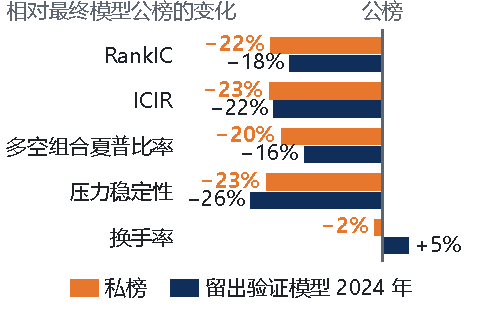
\includegraphics[height=4.95cm]{figures/fig_public_private_s.pdf}
    \column{0.40\textwidth}
    \vspace{0.12cm}
    \point{1}{波动没有变化}{逐截面 RankIC 标准差：公榜 0.0566，私榜 0.0568。}
    \point{2}{本地相邻两年同幅度}{留出验证模型 2024 年 ICIR 是 2023 年的 0.770 倍。}
    \point{3}{另一赛道同期回落}{因子赛道同一私榜区间 RankIC 为公榜的 0.768 倍。}
  \end{columns}
  \takeaway{只有一个私榜区间、日期未公布，两个赛道也不是独立样本，以上只作旁证。}
\end{frame}

% ---------------------------------------------------------------------
\gdef\chaplabel{备份 A3}
\begin{frame}{正则强度超过 \tn{0.1} 后 ICIR 明显下降}
  \begin{columns}[T]
    \column{0.58\textwidth}
    \vspace{0.05cm}
    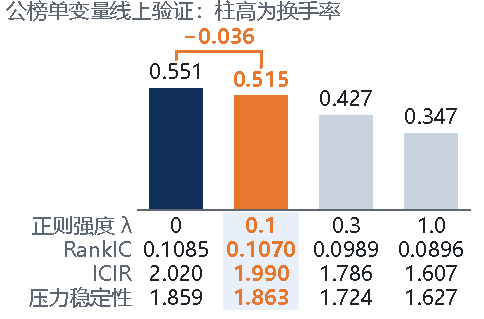
\includegraphics[height=4.95cm]{figures/fig_turnover_reg_s.pdf}
    \column{0.40\textwidth}
    \vspace{0.12cm}
    \point{1}{换手随强度单调下降}{本地 2023 年换手率由 0.573 降至 0.357，ICIR 由 2.078 降至 1.789。}
    \point{2}{强度 0.3、1.0 时 ICIR 明显下降}{ICIR 降至 1.786 和 1.607，压力稳定性降至 1.724 和 1.627。}
    \point{3}{全局换手惩罚已被否决}{惩罚所有股票相邻截面的预测变化，线上 RankIC −0.006。}
  \end{columns}
  \takeaway{公榜综合得分对 ICIR 与压力稳定性的敏感度高于换手率，强度 0.1 之后得分随之下降。}
\end{frame}

% ---------------------------------------------------------------------
\gdef\chaplabel{备份 A4}
\begin{frame}{神经网络读一档价量，树另读三档盘口}
  \vspace{0.05cm}
  {\small\renewcommand{\arraystretch}{1.3}\setlength{\tabcolsep}{5pt}
  \begin{tabularx}{\textwidth}{>{\raggedright\arraybackslash}p{3.2cm} >{\raggedright\arraybackslash}p{5.0cm} L}
    \headrow \thc{输入} & \thc{神经网络子模型} & \thc{梯度提升树子模型}\\
    1 分钟线，最近 64 根 & 一档价量，10 个字段 & 三档价量与委托笔数，25 个字段\\
    \ourrow 30 分钟窗口，18 个 & 价量 4 项、K 线形态 3 项、时段 & 同左，另加人工截面特征\\
    日线，之前 20 天 & 通道与 30 分钟窗口相同 & 之前 5 天的值与 20 天均值\\
    \ourrow 同伴画像，60 日 & 只用于计算股票间相似度 & 60 维原样输入\\
    使用方式 & 序列输入编码器 & 统一池化后共 1055 个特征\\
    \bottomrule
  \end{tabularx}}
  \par\vspace{0.3cm}
  \raggedright
  \begin{minipage}[t]{0.322\textwidth}
    \point{1}{输入不含三类内容}{官方风格暴露表、模型之前的输出、因子值。}
  \end{minipage}\hfill
  \begin{minipage}[t]{0.322\textwidth}
    \point{2}{截面特征现场计算}{价格位置、领先滞后等由原始行情现场计算。}
  \end{minipage}\hfill
  \begin{minipage}[t]{0.322\textwidth}
    \point{3}{输出与因子值互相隔离}{思路相互借鉴：部分特征选题受因子研究启发。}
  \end{minipage}
  \takeaway{全部输入在推理时由原始分钟行情现场计算；标签只在训练时读取。}
\end{frame}

% ---------------------------------------------------------------------
\gdef\chaplabel{备份 A5}
\begin{frame}{四个半年 RankIC 均不低于 \tn{0.0899}}
  \begin{columns}[T]
    \column{0.58\textwidth}
    \charthead{留出验证模型逐半年 RankIC（同结构、只训练到 2022 年）}
    \begin{tikzpicture}
      \begin{axis}[ybar, slidebar, width=8.4cm, height=5.0cm, bar width=30pt,
          ymin=0, ymax=0.133, enlarge x limits=0.16,
          xtick={1,2,3,4}, xticklabels={{2023 年\\上半年},{2023 年\\下半年},{2024 年\\上半年},{2024 年\\下半年}},
          point meta=y,
          nodes near coords={\pgfmathprintnumber[fixed,fixed zerofill,precision=4]{\pgfplotspointmeta}},
          nodes near coords style={font=\numfont\small,text=snavy}]
        \addplot[fill=snavy,draw=none,bar shift=0pt] coordinates {(1,0.1166) (2,0.1049) (4,0.0964)};
        \addplot[fill=sorange,draw=none,bar shift=0pt,
          nodes near coords style={font=\numfont\small\bfseries,text=sorange}] coordinates {(3,0.0899)};
      \end{axis}
    \end{tikzpicture}
    \column{0.40\textwidth}
    \vspace{0.02cm}
    \keynum{1.02}{四个半年换手率最大值与最小值之比；RankIC 为 1.30}
    \par\vspace{0.12cm}
    \point{1}{14:30 截面最强}{每个半年都最强，约为其他时段平均的 1.4～1.9 倍。}
    \point{2}{按日计 t 约 32}{2023 年 ICIR 2.057；未处理跨日自相关。}
  \end{columns}
  \takeaway{没有一个半年出现信号失效；换手率最稳，其余四项随行情环境同向变化。}
\end{frame}

% ---------------------------------------------------------------------
\gdef\chaplabel{备份 A6}
\begin{frame}{私榜模型由平台从零重训，训练可复现}
  \vspace{0.05cm}
  {\small\renewcommand{\arraystretch}{1.12}\setlength{\tabcolsep}{5pt}
  \begin{tabularx}{\textwidth}{>{\raggedright\arraybackslash}p{2.6cm} L}
    \headrow \thc{设置} & \thc{取值}\\
    训练区间 & 2020-01-01～2024-12-31，固定在脚本中；8,461,813 个股票-截面样本\\
    \ourrow 优化 & Adam，学习率 0.001，6 轮，不按验证集早停\\
    权重滑动平均 & 衰减 0.995；同配方两个随机种子的预测相关由 0.878 升至 0.941（2023 年）\\
    \ourrow 随机种子 & 第 k 个子模型用 42 + k；数据打乱、统计量抽样、聚类、树的抽样都固定\\
    训练耗时 & 7 个子模型顺序相加约 8.5 小时（两种硬件，不能外推平台耗时）\\
    \ourrow 冻结文件 & 权重 30,412,456 字节，低于平台 50 MB 上限\\
    \bottomrule
  \end{tabularx}}
  \par\vspace{0.18cm}
  \begin{minipage}[t]{0.485\textwidth}
    \point{1}{统计上等价}{浮点非确定性使权重不逐位相同；同配方换机器 RankIC 差约 0.001～0.002。}
  \end{minipage}\hfill
  \begin{minipage}[t]{0.485\textwidth}
    \point{2}{私榜用重训的模型评分}{私榜成绩不依赖本地训练的那份权重，说明训练流程在平台上可以复现。}
  \end{minipage}
  \takeaway{同一份脚本、同一组固定的配置与随机种子，从零训练得到统计上等价的模型。}
\end{frame}

\end{document}
